\scanpage{23}
$\mathcal G$ --- lequel opère donc sur $T$. Ceci donne naissance automatiquement \unsure{à|:}
\diagram{\begin{tikzcd}[ampersand replacement=\&,column sep=small]
\Phi:\unsure{\tau|\mathcal T}\&\unsure{\longrightarrow|\mathbin{-}}\&\operatorname{Hom}_{\mathrm{gr}}(T,\pi)\qquad\ldots
\end{tikzcd}}

Ceci dit, on a un hom du groupoïde $\langle\unsure{\tau|\mathcal T},\pi\rangle$ dans le groupoïde des rev. universels de $\Pi$, constant sur les objets et de valeur $\widetilde\Pi$ sur ceux-ci, qui envoie donc l'ens des flèches dans $\pi$ --- et qui pour $t,t'\in\unsure{\tau|\mathcal T}$, désignant par
\figure{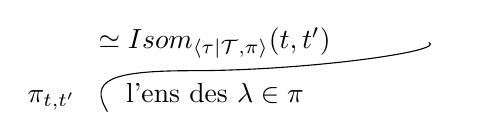
\begin{tikzpicture}[x=1cm,y=1cm]
\node[anchor=base west,inner sep=0pt] at (0,0) {$\pi_{t,t'}$};
\node[anchor=base west,inner sep=0pt] at (1.25,0) {l'ens des $\lambda\in\pi$};
\node[anchor=south west,inner sep=0pt] at (0.90,0.55) {\inserted{$\simeq\operatorname{Isom}_{\langle\unsure{\tau|\mathcal T},\pi\rangle}(t,t')$}};
\draw[thin] (1.02,-0.12) .. controls (0.78,0.28) and (1.05,0.40) .. (2.10,0.40) .. controls (3.55,0.40) and (5.35,0.65) .. (5.10,0.76);
\end{tikzpicture}}
tels que $\lambda t=t'$, est l'inclusion de $\pi_{t,t'}$ dans $\pi$. Ce foncteur
\diagram{\begin{tikzcd}[ampersand replacement=\&]
\langle\unsure{\tau|\mathcal T},\pi\rangle\arrow[r]\&
\begin{gathered}
\text{Cat des}\\
\text{rev. universels}\\
\text{de }\Pi\text{ égaux}\\
\text{\unsure{à|:} }\widetilde\Pi\\
\simeq(\text{un objet}\\
\text{et groupe d'isom---}\\
\pi)
\end{gathered}
\end{tikzcd}}
est évidemment compatible avec op. de $\unsure{\mathcal E|\Sigma}$ sur $\unsure{\Pi|\widetilde\Pi}$ donc sur $\pi\ldots.$
\mspage{22}
